\documentclass{beamer}

% packages
\usepackage[a-1b]{pdfx}
\usepackage{hyperref}
\usepackage{tikz}
\usepackage[labelformat=empty]{caption}
\usetikzlibrary{tikzmark, positioning}
\usetikzlibrary{decorations.markings}
\usetikzlibrary{arrows.meta}


% set up the presentation
\usetheme[subsection=false]{Darmstadt}
\usefonttheme[onlymath]{serif}

\title{A Perturbative Approach to the Ground State of Interacting Fermions in the Mean Field
Limit}
\author{
	Filippo Cozzi\\[1em]
	\small
	\begin{tabular}{l l} % 'l l' means two left-aligned columns
        Advisor:    & Dott. Matteo Gallone \\
        Co-advisor: & Prof. Niels Benedikter \\
    \end{tabular}
}
\date{July 17, 2026}

\begin{document}
\frame{\titlepage}

\section{The Fermi Gas}

\begin{frame}
	\frametitle{The interacting Fermi gas}
	The \textbf{Fermi gas} is a useful model in physics:
	\begin{itemize}
		\item<2-> nuclear matter (white dwarfs and neutron stars);
		\item<3-> condensed matter (electrons in crystalline structures);
		\item<4-> nuclear structure (shell structure of the atomic nucleus).
	\end{itemize}
	\vfill
	\uncover<5->{
		The behaviour of interacting fermions is not completely understood, even in
		the ground state: \textbf{approximate methods} are often used.
	}
	\vfill
	\begin{block}<6->{Objective}
		Mathematically rigorous analysis of the ground state energy of interacting fermions
		in the limit $N\to\infty$.
	\end{block}
\end{frame}

\section{Mean Field Limit}

\begin{frame}[t]
	\frametitle{Mean Field Limit}
	\small
	The $N$-body Hamiltonian on $L_{\mathrm{a}}^2(\mathbb{T}^{3N})$ is
	\vspace{-0.5em}
	\begin{align*}
		H_N = \sum_{i=1}^N-\hbar^2\Delta_i + \lambda\sum_{1\leq i<j\leq N}V(x_i-x_j)
	\end{align*}
	\vspace{-1.5em}
	\begin{columns}
		\begin{column}{.6\textwidth}
			\begin{itemize}
				\item<2-> Fermi energy $\epsilon(k_{\mathrm{F}})$ grows as
					$\mathcal{O}(N^{2/3})$\\
					$\implies$ \textbf{kinetic energy} grows as $\mathcal{O}(N^{5/3})$;
				\vfill\item<3-> number of interactions is $N(N-1)/2$\\
					$\implies$ \textbf{interaction energy} grows as $\mathcal{O}(N^2)$
					if $V$ is of order $\mathcal{O}(1)$.
			\end{itemize}
		\end{column}
		\begin{column}{.4\textwidth}
			\uncover<2->{
				\hfill
				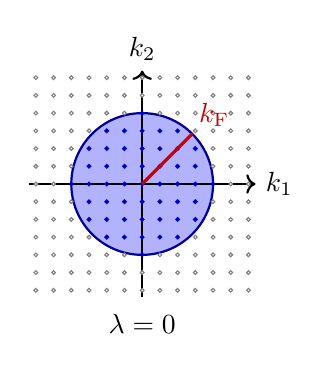
\begin{tikzpicture}[scale=0.45]
					% Draw the Fermi surface boundary (background)
					\draw[thick, blue!60!black, fill=blue!30] (0,0) circle (2.0);
					% Draw the axes
					\draw[->, thick] (-3.2,0) -- (3.2,0) node[right] {$k_1$};
					\draw[->, thick] (0,-3.2) -- (0,3.2) node[above] {$k_2$};
					% Generate the lattice of quantized momentum states
					% The step is 0.4, representing 2*pi/L
					\foreach \x in {-3.0,-2.5,...,3.0} {
						\foreach \y in {-3.0,-2.5,...,3.0} {
							% Calculate squared distance from origin (k^2 = kx^2 + ky^2)
							\pgfmathsetmacro{\rsq}{\x*\x + \y*\y}
							% Check if the state is inside or on the Fermi surface (k_F = 2.0)
							% Using 4.01 to account for minor floating point rounding
							\pgfmathparse{\rsq <= 4.01 ? 1 : 0}
							\ifnum\pgfmathresult=1
								% Filled state (inside Fermi ball)
								\filldraw[blue!80!black] (\x,\y) circle (1.5pt);
							\else
								% Empty state (outside Fermi ball)
								\draw[gray, fill=white] (\x,\y) circle (1.5pt);
							\fi
						}
					}
					% Draw the Fermi momentum vector (radius)
					\draw[-, very thick, red!80!black] (0,0) -- (1.414, 1.414) node[above right=-2pt] {$\boldsymbol{k_{\mathrm{F}}}$};
					\node [below=.5em, align=flush center] at (0,-3) {$\lambda=0$};
				\end{tikzpicture}
			}
		\end{column}
	\end{columns}
	\uncover<4->{
		\begin{block}{Mean field scaling}
			To have an extensive $H_N$ ($H_N\sim N$) in the limit $N\to\infty$, we define
			the \textbf{effective parameters}
			\vspace{-0.8em}
			\begin{align*}
				\tikzmarknode{semiclassical}{\hbar = N^{-1/3}}
				\quad\textrm{and}\quad
				\tikzmarknode{meanfield}{\lambda = N^{-1}}
			\end{align*}
		\end{block}
	}
	\only<5>{
		\begin{tikzpicture}[remember picture, overlay]
			\draw[red, thick]
				([shift={(-2pt,2pt)}]semiclassical.north west) rectangle
				([shift={(2pt,-2pt)}]semiclassical.south east);
			\draw[green, thick]
				([shift={(-2pt,2pt)}]meanfield.north west) rectangle
				([shift={(2pt,-2pt)}]meanfield.south east);
			\node[
				draw=red,
				very thick,
				fill=red!30,
				above=.7em of semiclassical,
				xshift=-3.5em,
				rounded corners
			] {semiclassical parameter};
			\node[
				draw=green,
				very thick,
				fill=green!30,
				above=.7em of meanfield,
				xshift=5em,
				rounded corners
			] {mean field coupling constant};
		\end{tikzpicture}
	}
\end{frame}

\begin{frame}
	\frametitle{Main Result}
	\small
	With ordinary second order perturbation theory
	\href{https://link.springer.com/article/10.1007/s00220-019-03654-7}
		{\footnotesize\textcolor{blue}{[Hainzl-Porta-Rexze, 2019]}}
	and then rigorous bosonization methods
	\href{https://link.springer.com/article/10.1007/s00222-021-01041-5}
		{\footnotesize\textcolor{blue}{[Benedikter-et-al, 2021]}}:
	\begin{align*}
		E^{\mathrm{gs}}_N = E^{\mathrm{HF}}_N + E^{\mathrm{RPA}}_N
		+ o\left(N^{-1/3}\right)\qquad\text{as}\;N\to\infty
	\end{align*}
	\uncover<2->{where}
	\begin{itemize}
		\item<2-> $E^{\mathrm{HF}}_N=\mathcal{O}(N)+\mathcal{O}(1)$ is the
			\textbf{Hartree-Fock (HF)} term;
		\item<3-> $E^{\mathrm{RPA}}_N=\mathcal{O}(N^{-1/3})$ from
			\textbf{Random Phase Approximation (RPA)}.
	\end{itemize}
	\vspace{-0.4em}
	\begin{block}<4->{Theorem: leading order contribution}
		As $N\to\infty$, the leading order contribution to $E^{\mathrm{gs}}_N$ is
		\begin{align*}
			E^{\mathrm{HF}}_N = \mathcal{O}(N) + \mathcal{O}(1).
		\end{align*}
	\end{block}
	\uncover<5->{\textbf{Main novelty}: The use of perturbation theory with QFT methods.}
	\vfill
	\uncover<6->{\textbf{Long-term objective}:To understand the connection between
		bosonization and QFT methods.}
\end{frame}

\section{Sketch of the proof}

\begin{frame}
	\frametitle{Sketch of the proof: definitions}
	\textbf{Second quantized} Hamiltonian:
	\alt<1-5>{
		\begin{align*}
			H = \sum_{k\in\mathbb{Z}^3} (\hbar^2\vert k\vert^2 - \mu)a^*_k a_k
			\vphantom{\underbrace{\sum_{k\in\mathbb{Z}^3} (\hbar^2\vert k\vert^2 - \mu)a^*_k a_k}_{H_0}}
			+ \lambda \sum_{p,q,k\in\mathbb{Z}^3} \hat{V}(k)a^*_{p-k}a^*_{q+k} a_q a_p
		\end{align*}
	}{
		\begin{align*}
			H = {\underbrace{\sum_{k\in\mathbb{Z}^3} (\hbar^2\vert k\vert^2 - \mu)a^*_k a_k}_{H_0}}
			+ \lambda \sum_{p,q,k\in\mathbb{Z}^3} \hat{V}(k)a^*_{p-k}a^*_{q+k} a_q a_p
		\end{align*}
	}
	\uncover<2->{
		where
		\begin{itemize}
			\item<2-> $\mu$ is the chemical potential fixed by $N$;
			\item<3-> $V$ depends only on distances: $V(x_i-x_j)=V(\vert x_i-x_j\vert)$;
			\item<4-> $\hat{V}$ has compact support.
		\end{itemize}
	}
	\vfill
	\uncover<5-6>{
		A \textbf{thermal equilibrium state} at (inverse) temperature $\beta$ is
		\begin{align*}
			\rho = \frac{e^{-\beta H}}{Z}, \quad\text{with}\; Z = \mathrm{Tr}(e^{-\beta H})
		\end{align*}
		and expectations are $\langle\,\cdot\,\rangle_{\beta,H} = \mathrm{Tr}(\,\cdot\,\rho)$.
	}
\end{frame}

\begin{frame}
	\frametitle{Sketch of the proof: toolbox}
	\small
	The \textbf{free energy} is $F = -\frac{\log(Z)}{\beta}$, and $E^{\mathrm{gs}}_N=
	\lim_{\beta\to\infty}F$.
	\vfill
	\begin{block}<2->{}
		\textbf{Duhamel's formula} at second order for $\log(Z)$:
		\begin{align*}
			&\log\,\mathrm{Tr}\,e^{-\beta H}=
			\log\,\mathrm{Tr}\,e^{-\beta H_0} - \lambda\beta\langle V\rangle_{\beta,H_0}\\
			&\quad+ \lambda^2 \int_0^\beta\int_0^\tau
			\left[\langle V(\tau')V(\tau)\rangle_{\beta,H_0} - \langle V(\tau')\rangle_{\beta,H_0}\langle V(\tau)\rangle_{\beta,H_0}\right]
			\mathrm{d}\tau'\mathrm{d}\tau
		\end{align*}
	\end{block}
	\vfill
	\begin{block}<3->{}
		\textbf{Wick's theorem}: $H_0 = \sum_{k}\epsilon_k a^*_ka_k$ and $A_j=a^*_j,a_j$, then
		\begin{align*}
			\langle A_1\cdots A_{2n}\rangle_{\beta,H_0} &=
			\sum_{\sigma\in P_{2n}}(-1)^\sigma\prod_{j=1}^{2n-1}\langle A_{\sigma(j)}A_{\sigma(j+1)}\rangle_{\beta,H_0}\\
			\langle A_1\cdots A_{2n-1}\rangle_{\beta,H_0} &= 0
		\end{align*}
		where $P_{2n}$ is the set of \textbf{pairings} of $2n$ elements.
	\end{block}
\end{frame}

\begin{frame}
	\frametitle{Sketch of the proof: Feynman diagrams}
	Diagrammatically:
	\begin{gather*}
		\uncover<2->{
			G_{k,k'}(\tau,\tau') =
			\langle a^*_k(\tau)a_{k'}(\tau') \rangle_{\beta,H_0}
			= 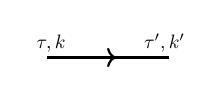
\begin{tikzpicture}[scale=.6, baseline=(current bounding box.south)]
				\node (a) at (-1.5,0) {} node[scale=0.7] at (-1.2,0.3) {$\tau,k$};
				\node (b) at ( 1.5,0) {} node[scale=0.7] at ( 1.2,0.3) {$\tau',k'$};
				\begin{scope}[very thick, decoration={
						markings,
						mark=at position 0.57 with {\arrow{>}}}
					]
					\draw[black, thick, postaction={decorate}] (a) -- (b);
				\end{scope}
			\end{tikzpicture}
		}
		\\
		\uncover<3->{
			\sum_{p,q,k}\hat{V}(k)a^*_{p-k}a^*_{q+k}a_qa_p =
			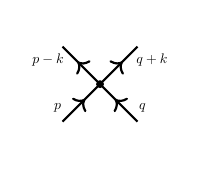
\begin{tikzpicture}[scale=.6, baseline=(current bounding box.center)]
				\node (a) at (-1, 1) {} node[scale=0.5] at (-1.1, 0.5) {$p-k$};
				\node (b) at ( 1, 1) {} node[scale=0.5] at ( 1.1, 0.5) {$q+k$};
				\node (c) at (-1,-1) {} node[scale=0.5] at (-0.9,-0.5) {$p$};
				\node (d) at ( 1,-1) {} node[scale=0.5] at ( 0.9,-0.5) {$q$};
				\begin{scope}[very thick, decoration={
						markings,
						mark=at position 0.6 with {\arrow{>}}}
					]
					\draw[black, thick, postaction={decorate}] (0,0) -- (a);
					\draw[black, thick, postaction={decorate}] (0,0) -- (b);
					\draw[black, thick, postaction={decorate}] (c) -- (0,0);
					\draw[black, thick, postaction={decorate}] (d) -- (0,0);
				\end{scope}
				\filldraw[black] (0,0) circle (2pt);
			\end{tikzpicture}
		}
	\end{gather*}
	\uncover<4->{
		The first order contribution is:
	}
	\begin{align*}
		\uncover<4->{
			\lim_{\beta\to\infty}\lambda\langle V\rangle_{\beta,H_0}
			&=
		}
		\uncover<5->{
			\lim_{\beta\to\infty}\lambda\left(
			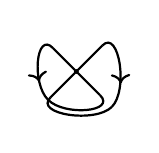
\begin{tikzpicture}[scale=.3, baseline=(current bounding box.center)]
				\node[shape=coordinate] (a) at (-1, 1) {};
				\node[shape=coordinate] (b) at ( 1.1, 1.1) {};
				\node[shape=coordinate] (c) at (-1.1,-1.1) {};
				\node[shape=coordinate] (d) at ( 1,-1) {};
				\coordinate (A) at (-1.2,-1.2);
				\coordinate (B) at ( 1.5,-1.5);
				\draw[black, thick] (0,0) -- (a);
				\draw[black, thick] (0,0) -- (b);
				\draw[black, thick] (0,0) -- (c);
				\draw[black, thick] (0,0) -- (d);
				\filldraw[black] (0,0) circle (2pt);
				\begin{scope}[very thick, decoration={
						markings,
						mark=at position 0.7 with {\arrow{>}}}
					]
					\draw[black, thick, postaction={decorate}] (a) .. controls +(135:1) and +(135:1) .. (A);
					\draw[black, thick]                        (A) .. controls +(315:1) and +(315:1) .. (d);
				\end{scope}
				\begin{scope}[very thick, decoration={
						markings,
						mark=at position 0.45 with {\arrow{<}}}
					]
					\draw[black, thick]                        (c) .. controls +(225:1) and +(225:1) .. (B);
					\draw[black, thick, postaction={decorate}] (B) .. controls +( 45:1) and +( 45:1) .. (b);
				\end{scope}
			\end{tikzpicture}
			+
			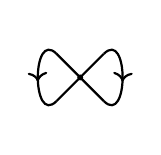
\begin{tikzpicture}[scale=.3, baseline=(current bounding box.center)]
				\node[shape=coordinate] (a) at (-1, 1) {};
				\node[shape=coordinate] (b) at ( 1, 1) {};
				\node[shape=coordinate] (c) at (-1,-1) {};
				\node[shape=coordinate] (d) at ( 1,-1) {};
				\draw[thick] (0,0) -- (a);
				\draw[thick] (0,0) -- (b);
				\draw[thick] (0,0) -- (c);
				\draw[thick] (0,0) -- (d);
				\filldraw[black] (0,0) circle (.1);
				\begin{scope}[very thick, decoration={
						markings,
						mark=at position 0.55 with {\arrow{>}}}
					]
					\draw[thick, postaction={decorate}] (a) .. controls +(135:1.5) and +(225:1.5) .. (c);
					\draw[thick, postaction={decorate}] (b) .. controls +( 45:1.5) and +(315:1.5) .. (d);
				\end{scope}
			\end{tikzpicture}
			\right)\\
		}
		\uncover<6->{
			&= N^{-1}\sum_{\substack{k\in\mathbb{Z}^3,\;p\in B_{\mathrm{F}}:\\p-k\in B_{\mathrm{F}}}}
			\left(\hat{V}(0)-\hat{V}(k)\right)\\
			&= \mathcal{O}(N) + \mathcal{O}(1).
		}
	\end{align*}
\end{frame}

\section{Second Order Contributions}

\begin{frame}
	\frametitle{Future perspective: a first look at second order}
	\small
	At second order, the \textbf{connected Feynman diagrams} are split into two possible
	topologies:
	\vspace{-1.3em}
	\begin{figure}[h]
		\begin{minipage}[t]{.43\textwidth}
			\raggedleft
			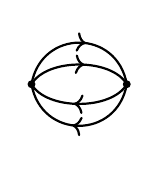
\begin{tikzpicture}[scale=.55, baseline=(current bounding box.center)]
				\node[shape=coordinate] (a) at (-1.1,0) {};
				\node[shape=coordinate] (b) at ( 1.1,0) {};
				\begin{scope}[very thick, decoration={
						markings,
						mark=at position 0.55 with {\arrow{>}}}
					]
					\filldraw[] (-1.1,0) circle (.05);
					\filldraw[] ( 1.1,0) circle (.05);
					\draw[thick, postaction={decorate}] (a) .. controls +( 80:1.3) and +(100:1.3) .. (b);
					\draw[thick, postaction={decorate}] (b) .. controls +(260:1.3) and +(280:1.3) .. (a);
					\draw[thick, postaction={decorate}] (a) .. controls +( 60:0.7) and +(120:0.7) .. (b);
					\draw[thick, postaction={decorate}] (b) .. controls +(240:0.7) and +(300:0.7) .. (a);
				\end{scope}
			\end{tikzpicture}
		\end{minipage}
		\hfill
		\begin{minipage}[t]{.48\textwidth}
			\raggedright
			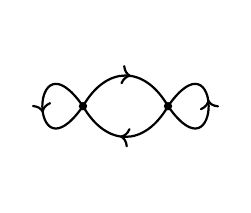
\begin{tikzpicture}[scale=.6, baseline=(current bounding box.center)]
				\node[shape=coordinate] (a) at (-0.9,0) {};
				\node[shape=coordinate] (b) at ( 0.9,0) {};
				\begin{scope}[very thick, decoration={
						markings,
						mark=at position 0.55 with {\arrow{>}}}
					]
					\filldraw[] (-0.9,0) circle (.05);
					\filldraw[] ( 0.9,0) circle (.05);
					\draw[thick, postaction={decorate}] (a) .. controls +(125:2) and +(235:2) .. (a);
					\draw[thick, postaction={decorate}] (b) .. controls +(305:2) and +( 55:2) .. (b);
					\draw[thick, postaction={decorate}] (a) .. controls +( 60:1) and +(120:1) .. (b);
					\draw[thick, postaction={decorate}] (b) .. controls +(240:1) and +(300:1) .. (a);
				\end{scope}
			\end{tikzpicture}
		\end{minipage}
	\end{figure}
	\uncover<2->{
		However, they contain unphysical results, like the \textbf{tadpole divergence}:
	}
	\begin{align*}
		\uncover<2->{
			\lim_{\beta\to\infty}\frac{\beta}{2}\left(
			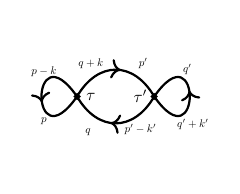
\begin{tikzpicture}[scale=.35, baseline=(current bounding box.center)]
				\node[shape=coordinate] (a) at (-1.4,0) {} node[scale=.6] at (-0.9,0) {$\tau$};
				\node[shape=coordinate] (b) at ( 1.4,0) {} node[scale=.6] at ( 0.9,0) {$\tau'$};
				\node[scale=0.4] (m1) at (-2.6, 0.9) {$p-k$};
				\node[scale=0.4] (m2) at (-0.9, 1.2) {$q+k$};
				\node[scale=0.4] (m3) at (-2.6,-0.9) {$p$};
				\node[scale=0.4] (m4) at (-1.0,-1.3) {$q$};
				\node[scale=0.4] (n1) at ( 2.6, 1.0) {$q'$};
				\node[scale=0.4] (n2) at ( 1.0, 1.2) {$p'$};
				\node[scale=0.4] (n3) at ( 2.8,-1.0) {$q'+k'$};
				\node[scale=0.4] (n4) at ( 0.9,-1.2) {$p'-k'$};
				\begin{scope}[very thick, decoration={
						markings,
						mark=at position 0.55 with {\arrow{>}}}
					]
					\filldraw[] (a) circle (.05);
					\filldraw[] (b) circle (.05);
					\draw[thick, postaction={decorate}] (a) .. controls +(125:3) and +(235:3) .. (a);
					\draw[thick, postaction={decorate}] (b) .. controls +(305:3) and +( 55:3) .. (b);
					\draw[thick, postaction={decorate}] (a) .. controls +( 60:1.5) and +(120:1.5) .. (b);
					\draw[thick, postaction={decorate}] (b) .. controls +(240:1.5) and +(300:1.5) .. (a);
				\end{scope}
			\end{tikzpicture}\right)
		}
		\uncover<3->{
			&= \lim_{\beta\to\infty}\left( -\frac{\beta}{2}\sum_{p,q,k}\hat{V}(0)^2n_q^2\tikzmarknode{fermidirac}{n_p}n_{k} \right)\\
		}
		\uncover<4->{
			&= -\infty
		}
	\end{align*}
	\uncover<3->{
		\begin{tikzpicture}[remember picture, overlay]
			\node[
				draw=red,
				fill=red!0,
				thick,
				below=1.5em of fermidirac,
				rounded corners
				] (comment) {$n_p = n_{\mathrm{F}}(\epsilon_p)$};
			\draw[red,thick,->] (comment.north) -- ([shift={(0,-.3em)}]fermidirac.south);
		\end{tikzpicture}
	}
	\vspace{-1em}
	\begin{block}<5->{Remark}
		Perturbatively, the RPA is understood as a partial resummation \textbf{at all orders}.
		Removing divergences might be highly non-trivial!
	\end{block}
\end{frame}

\section*{}

\begin{frame}[plain]
	\frametitle{Conclusion}
	\begin{block}{}
		We successfully employed QFT methods to re-derive the first order correction to
		the ground state energy of an interacting Fermi gas in the mean field limit.
	\end{block}
	\vfill
	\uncover<2->{\textbf{Short-term future perspective}:}
	\begin{itemize}
		\item<3-> $\tau$-ordered Grassmann integrals;
		\item<4-> Matsubara frequencies;
		\item<5-> order-by-order identification of Feynman diagrams and Wick contractions.
	\end{itemize}
	\vfill
	\uncover<2->{\textbf{Ultimate goal}:}
	\uncover<6->{to take the proof of the $N$-scaling of the ground state energy to all
	orders in perturbation theory.}
\end{frame}

\begin{frame}[plain]
	\centering
	\vspace{2.0em}
	\Huge Thank you!
\end{frame}

%\begin{frame}[plain]
%	\centering
%	\vspace{2.0em}
%	\Huge
%	\begin{align*}
%		\int_E f\,\mathrm{d}\mu \; \neq \; \int_E f\,d\mu
%	\end{align*}
%\end{frame}

\end{document}
